\documentclass[11pt,a4paper]{article}
\usepackage[utf8]{inputenc}\usepackage[T1]{fontenc}
\usepackage{amsmath, amssymb, amsthm}
\usepackage[margin=1in]{geometry}
\usepackage{hyperref}\usepackage{mathrsfs}\usepackage{graphicx}\usepackage{booktabs}
\hypersetup{hidelinks}
\newtheorem{proposition}{Proposition}
\newtheorem{definition}{Definition}
\theoremstyle{remark}\newtheorem{remark}{Remark}

\title{\Large \textbf{The Second Moment of $\omega$ under Twin-Centre\\
Conditioning on the $6N$ Skeleton:\\ A Near-Poisson Tilt with Conserved Dispersion}}
\author{Ruqing Chen\\
\small GUT Geoservice Inc., Montreal, Quebec, Canada\\
\small \texttt{ruqing@hotmail.com}}
\date{\today}

\begin{document}
\maketitle

\begin{abstract}
Every earlier part of this programme worked with \emph{first} moments: the mean
enrichment of twin centres as a function of $\omega_{>3}(N)$, the number of distinct
prime factors of the centre exceeding $3$. The \emph{second} moment---the
Erd\H{o}s--Kac-type variance, and how it responds to conditioning on a centre being
a twin centre---was left open. We close it empirically. Sieving all centres up to
$6N=6\times10^8$ ($2{,}166{,}300$ twin centres), we measure the full distribution of
$\omega_{>3}(N)$ over all centres and over twin centres. Twin-conditioning shifts the
mean by a saturating amount ($+0.171\to+0.215$ as $6N$ runs $1.5\times10^6\to
6\times10^8$, decelerating toward a finite, small-prime-dominated limit) and
inflates the variance by a stable factor $1.104\pm0.005$, while the dispersion ratio
$\mathrm{Var}/\mathrm{mean}$ is \emph{conserved}: its twin-to-all ratio is
$1.011\pm0.004$ across two and a half orders of magnitude. We interpret this as a
\emph{near-Poisson tilt}: writing $\omega$ as a sum of nearly independent
Bernoulli indicators $\mathbf 1[q\mid N]$, the twin weight $\prod_{q\mid N}q/(q-2)$
nudges each inclusion probability up by $\approx2/(q(q-2))$, a convergent
small-prime-dominated series that shifts the mean to a finite limit and rescales
mean and variance nearly in step. The Erd\H{o}s--Kac dispersion thus survives
conditioning. We are explicit: this is new \emph{to the programme}, not new
mathematics---it confirms, and does not supersede, classical Erd\H{o}s--Kac. We also
record a clarification that ties off a separate thread: the ``annihilation lattice''
of Part~XXI is exactly the classical Hardy--Littlewood admissibility condition.
\end{abstract}

\section{Introduction}
The arithmetic-geodynamics programme has repeatedly used the stratification of
centres $N$ by $\omega_{>3}(N)$, the count of distinct prime factors $>3$: twin
centres are enriched at high $\omega$ (the ``wind tunnel'' of Volume~I and the
kinetics of Part~XXIII)~\cite{ChenXVII,ChenXXIII}. Every such statement was a
statement about the mean. The distribution itself---in particular its variance, the
object of the Erd\H{o}s--Kac theorem~\cite{ErdosKac}---was never measured here, and
the variance was flagged as open throughout.

The classical Erd\H{o}s--Kac theorem says $\omega(n)$ is asymptotically normal with
mean and variance both $\sim\ln\ln n$. The programme-specific question is what
happens to this distribution when we \emph{condition} on $N$ being a twin centre.
The first-moment results guarantee the mean moves up; they say nothing about the
spread. This paper measures both, at scale.

\section{Method}
For a centre $N$ let $\omega_{>3}(N)$ be the number of distinct primes $p>3$
dividing $N$ (i.e.\ $\omega(N)$ minus the indicators of $2\mid N$ and $3\mid N$). A
centre is a \emph{twin centre} if $6N-1$ and $6N+1$ are both prime. We sieve all
centres $N\le 10^8$ (so $6N\le6\times10^8$), computing $\omega_{>3}(N)$ by a
distinct-prime-factor sieve and twin-centre membership from a prime sieve to
$6\times10^8$, and we tabulate the empirical distribution of $\omega_{>3}$ over all
centres and over the $2{,}166{,}300$ twin centres, at a ladder of cutoffs.

\section{Results}
\paragraph{The two distributions.} Figure~\ref{fig:dist} shows the distribution of
$\omega_{>3}(N)$ over all centres versus over twin centres at $6N=6\times10^8$. The
twin distribution is shifted right and modestly widened; the per-$\omega$
enrichment $P(\omega\mid\text{twin})/P(\omega\mid\text{all})$ rises monotonically
across $\omega=1,\dots,5$, the distributional face of the multiplicative
wind-tunnel enrichment.

\begin{figure}[h]\centering
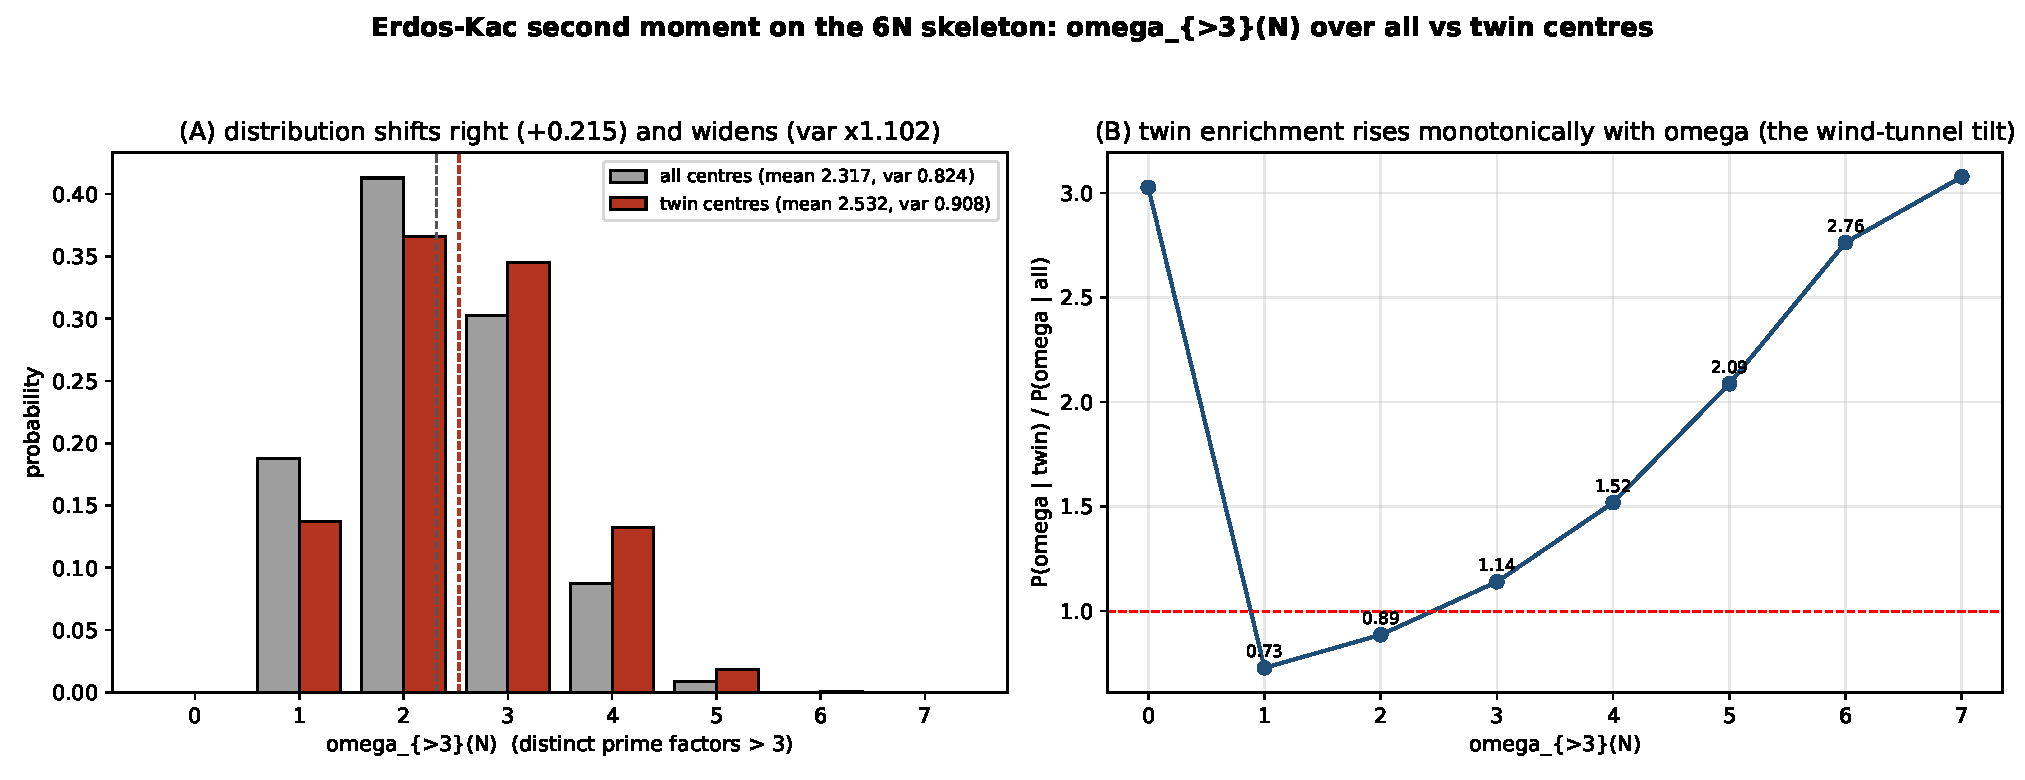
\includegraphics[width=0.97\textwidth]{fig_omega_variance.pdf}
\caption{(A) Distribution of $\omega_{>3}(N)$ over all centres vs.\ twin centres at
$6N=6\times10^8$: a rightward mean shift and a modest widening. (B) The per-$\omega$
enrichment ratio rises monotonically over $\omega=1$--$5$ (the wind-tunnel tilt);
$\omega=0,6$ are low-count edge bins.}
\label{fig:dist}
\end{figure}

\paragraph{Moments across scale.} Table~\ref{tab:scale} collects the first two
moments at six cutoffs. Two trends are clean and stable
(Fig.~\ref{fig:trend}). First, the \emph{mean shift}
$\langle\omega\rangle_{\rm twin}-\langle\omega\rangle_{\rm all}$ grows but
decelerates sharply, approaching a finite limit $\approx0.21$--$0.22$; it does not
track $\ln\ln(6N)$. Second, the \emph{dispersion ratio} $\mathrm{Var}/\mathrm{mean}$
rises with scale for both populations (finite-size approach to the Erd\H{o}s--Kac
value), but the twin-to-all ratio of $\mathrm{Var}/\mathrm{mean}$ stays at
$1.011\pm0.004$, and the variance ratio at $1.104\pm0.005$, over the full range.

\begin{table}[h]\centering
\begin{tabular}{rccccc}
\toprule
$6N_{\max}$ & $\ln\ln(6N_{\max})$ & mean shift & Var ratio (twin/all)
 & $(\mathrm{V/m})_{\rm all}$ & $(\mathrm{V/m})_{\rm twin}$\\
\midrule
$1.5\times10^6$ & $2.655$ & $+0.1710$ & $1.097$ & $0.2896$ & $0.2916$\\
$6\times10^6$   & $2.748$ & $+0.1845$ & $1.109$ & $0.3066$ & $0.3117$\\
$3\times10^7$   & $2.846$ & $+0.1995$ & $1.111$ & $0.3252$ & $0.3303$\\
$1\times10^8$   & $2.913$ & $+0.2085$ & $1.105$ & $0.3380$ & $0.3414$\\
$3\times10^8$   & $2.971$ & $+0.2120$ & $1.102$ & $0.3489$ & $0.3518$\\
$6\times10^8$   & $3.006$ & $+0.2149$ & $1.102$ & $0.3554$ & $0.3585$\\
\bottomrule
\end{tabular}
\caption{First two moments of $\omega_{>3}(N)$ over all vs.\ twin centres, at six
cutoffs. The mean shift saturates; the variance ratio and the dispersion ratio are
scale-stable.}
\label{tab:scale}
\end{table}

\begin{figure}[h]\centering
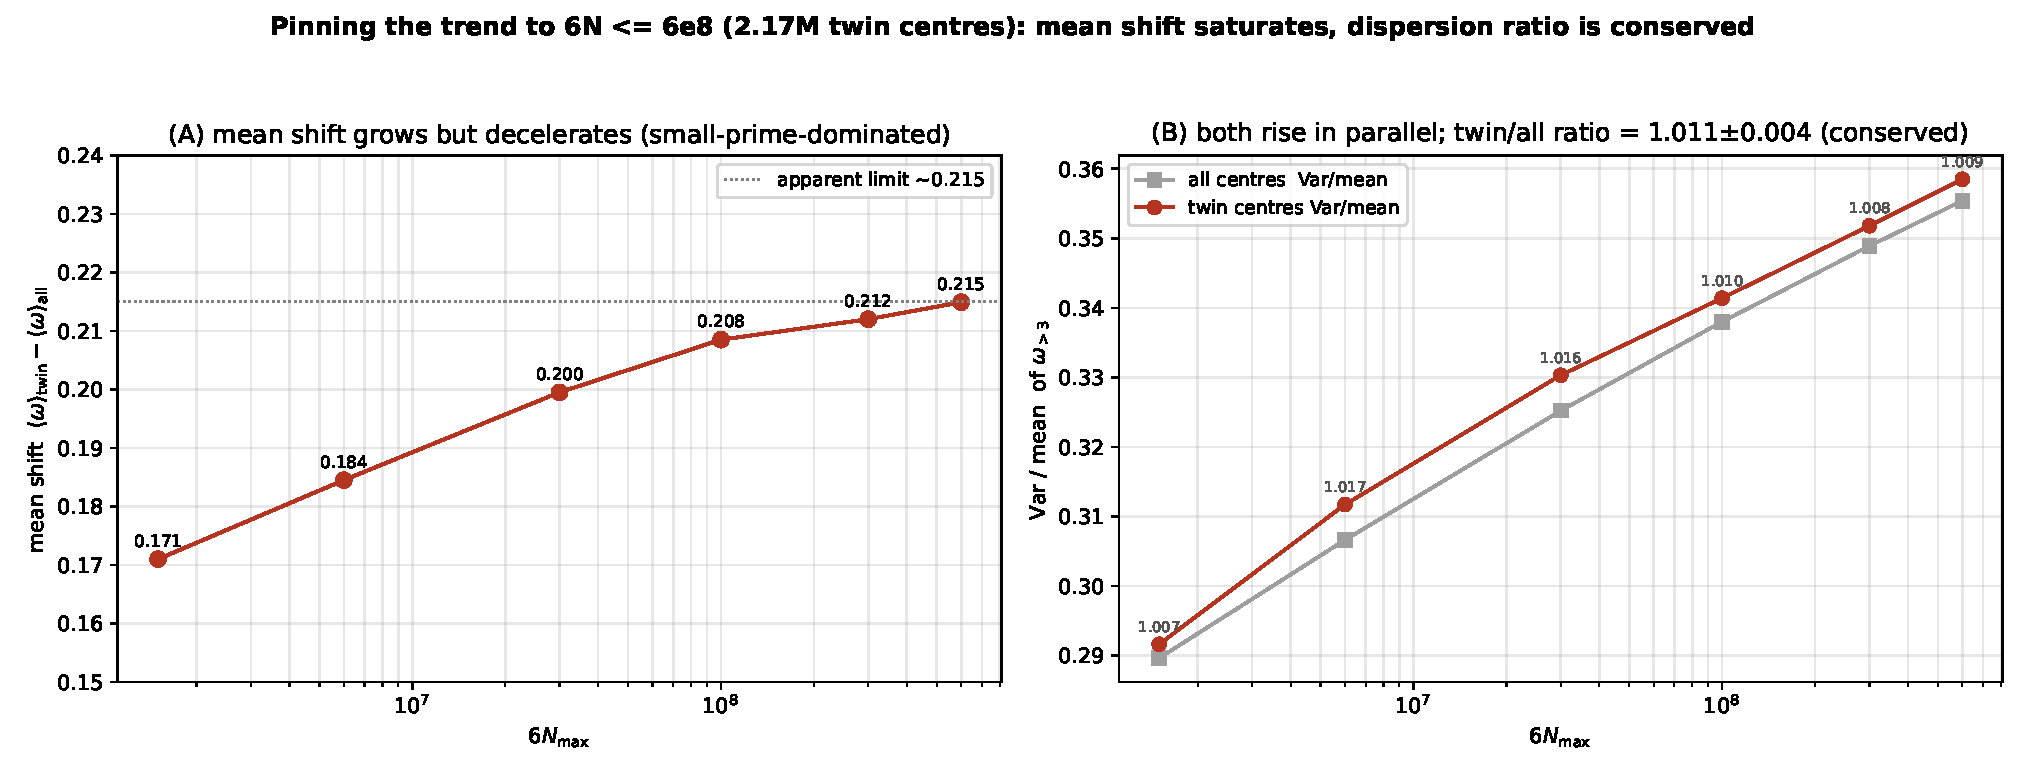
\includegraphics[width=0.97\textwidth]{fig_omega_trend.pdf}
\caption{(A) The mean shift grows but decelerates toward an apparent limit
$\approx0.215$ (small-prime-dominated). (B) $\mathrm{Var}/\mathrm{mean}$ rises in
parallel for both populations; their ratio is conserved at $1.011\pm0.004$ across
$6N=1.5\times10^6$ to $6\times10^8$.}
\label{fig:trend}
\end{figure}

\section{Interpretation: a near-Poisson tilt}
Write $\omega_{>3}(N)=\sum_{q>3}\mathbf 1[q\mid N]$, a sum of nearly independent
Bernoulli indicators with $\Pr[q\mid N]=1/q$. The two-centre enrichment established
earlier weights a centre by
$w(N)=\prod_{q\mid N,\,q>3} q/(q-2)$~\cite{ChenXXIII}, so conditioning on a twin
centre nudges each inclusion probability from $1/q$ toward $\sim1/(q-2)$.

\paragraph{Mean shift is a convergent small-prime sum.} To leading order the shift
in the mean is
\begin{equation}
  \langle\omega\rangle_{\rm twin}-\langle\omega\rangle_{\rm all}
  \;\approx\;\sum_{q>3}\Big(\tfrac{1}{q-2}-\tfrac1q\Big)
  =\sum_{q>3}\frac{2}{q(q-2)},
\end{equation}
a convergent series dominated by the smallest primes ($q=5$ alone contributes
$\tfrac{2}{15}=0.133$; $q=7$ adds $0.057$). The leading-order value $\approx0.26$
overestimates the measured shift because it ignores the normalisation by
$\mathbb{E}[w]$ and inter-prime correlations; the measured shift approaches a limit
of this order \emph{from below}, which is exactly the observed saturation: the shift
is set by a handful of small primes and cannot grow like $\ln\ln$.

\paragraph{Dispersion is conserved.} For a sum of Bernoulli$(p_q)$ indicators,
$\mathrm{mean}=\sum p_q$ and $\mathrm{Var}=\sum p_q(1-p_q)$, so
$\mathrm{Var}/\mathrm{mean}=1-\big(\sum p_q^2\big)/\big(\sum p_q\big)$. The twin tilt
raises the $p_q$ only slightly, and only for $q>3$, so this ratio moves by about a
percent---precisely the measured $(\mathrm{V/m})_{\rm twin}/(\mathrm{V/m})_{\rm
all}=1.011\pm0.004$. The tilt rescales mean and variance nearly in step: it is, to
good approximation, a \emph{near-Poisson tilt}, and the Erd\H{o}s--Kac dispersion
survives conditioning intact.

\section{A clarification: the annihilation lattice is classical admissibility}
A separate thread of Volume~II asked for the ``general $k$-body tiling spectrum.''
We record here, to prevent a misreading, that the tiling/annihilation criterion of
Part~XXI~\cite{ChenXXI}---a configuration of constellations has zero joint density
iff their shifted dead-residue sets cover $\mathbb{Z}/q$ for some prime $q$---is
\emph{identical} to the classical Hardy--Littlewood admissibility
condition~\cite{HL}: a set of offsets is inadmissible iff it occupies every residue
modulo some prime. For instance $\{0,2,4\}$ covers $\mathbb{Z}/3$ (inadmissible $=$
``annihilates''), while $\{0,2,6\}$ does not (admissible). The annihilation lattice
is thus the complement of the admissible set, and it connects to Erd\H{o}s covering
systems; mapping it on the skeleton recovers known combinatorics in new
coordinates, and we make no claim of a new criterion.

\section{Conclusion}
Measuring the second moment closes a question the programme had left open since
Volume~I. Conditioning on a twin centre acts as a near-Poisson tilt of the
$\omega_{>3}$ distribution: it shifts the mean by a saturating, small-prime-dominated
amount ($\to\approx0.21$--$0.22$), inflates the variance by a stable factor $1.104$,
and conserves the dispersion ratio $\mathrm{Var}/\mathrm{mean}$ to about a percent
across two and a half orders of magnitude. The Erd\H{o}s--Kac spread is preserved
under conditioning, merely rescaled. We state the scope plainly: this is a new
measurement \emph{for this programme}, not a new theorem; it confirms classical
Erd\H{o}s--Kac rather than extending it, and it makes no claim about the infinitude
of twins or any constellation. Together with the admissibility clarification, it
ties off the two open threads of Volume~II.

\paragraph{Data and code availability.}
The sieve experiment (to $6N=6\times10^8$), the figures, and a verifier (small-scale
moments and the admissibility$=$covering equivalence) are openly available at
\url{https://github.com/Ruqing1963/6N-omega-variance}~\cite{repo}.

\begin{thebibliography}{9}
\bibitem{ErdosKac} P.~Erd\H{o}s, M.~Kac, \emph{The Gaussian law of errors in the
theory of additive number theoretic functions}, Amer.\ J.\ Math.\ \textbf{62}
(1940), 738--742.
\bibitem{HL} G.~H.~Hardy, J.~E.~Littlewood, \emph{Some problems of `Partitio
Numerorum'; III}, Acta Math.\ \textbf{44} (1923), 1--70.
\bibitem{ChenXVII} R.~Chen, \emph{Arithmetic geodynamics on the $6N$ skeleton}
(Part~XVII), Zenodo, doi:10.5281/zenodo.20541575 (2026).
\bibitem{ChenXXI} R.~Chen, \emph{The irreducible three-body congruence correlation
and the annihilation lattice} (Part~XXI), Zenodo, doi:10.5281/zenodo.20584909 (2026).
\bibitem{ChenXXIII} R.~Chen, \emph{Phase transition kinetics and topological event
horizons at extreme $\omega$} (Part~XXIII), Zenodo, doi:10.5281/zenodo.20586919 (2026).
\bibitem{Review} R.~Chen, \emph{Arithmetic geodynamics on the $6N$ skeleton: a
review of Parts I--XIX}, Zenodo, doi:10.5281/zenodo.20585301 (2026).
\bibitem{repo} R.~Chen, \emph{The second moment of $\omega$ under twin-centre
conditioning on the $6N$ skeleton} (Part~XXVI),
\url{https://github.com/Ruqing1963/6N-omega-variance} (2026).
\end{thebibliography}

\end{document}
